This chapter includes the design decision taken while implementing the \acrfull{wdias}, and how is the system got adapted from the systems analyzed in Chapter \ref{ch:literature}, then how is it trying to propose a better system with overcoming the issues.
In the section \ref{se:high_level_design}, it give a brief disussion on how the weather forecasting is happening, and why it need to interact with multiple data formats.
Then following subsections define few termelogy which are using in the \acrshort{wdias}, and scope of the thesis.
Following section \ref{se:architectural_decisions} that we evolve over while designing and implementing the \acrshort{wdias}.
The section \ref{se:microservice} gives better understanding of the microservice architectural concepts follows while implementing the \acrshort{wdias}.
Then the reason behind developing Heirarchital Database and technologies use for that discussed in the section \ref{se:db_struct}.
Throw out the section \ref{se:data_preprocess} discussed about how the \acrshort{wdias} enable for data preprocessing and adding capabilities via concept of Extensions.
Last section \ref{se:query} includes details on how to perform timeseries search and geo based queries.

%%%%%%%%%%%%%%%%%%%%%%%%%%%%%%%%%%%%%%%%%%%%%%%%%%%%%%%%%%%%%%%%%%%%%%%%%%%%%%%%
\section{High-level Design}
\label{se:high_level_design}

In order to get overall idea on the flow of weather prediction, lets look into one of flows using in \acrshort{curw} \cite{CUrWSL2017SL}.
\begin{itemize}
    \item Extract GRIB WRF model data to netCDF
    \item From netCDF to CSV of each location data, then feed to HEC-HMS and get the output as CSV
    \item CSV + Rain cell Grid feed into the FLO2D, and get the water level as Grid ASCII files after completion of simulation
    \item Upload ASCII files to ArcGIS create Raster files, then use for the LOSS Estimation
\end{itemize}
When looked into the above flow, it clear understanding on multiple data formats using while weather predictions.
Other than that, in order to correct the model outputs, it required to collect real time data such as;
\begin{itemize}
    \item Automated weather station sending data in higher frequent intervals via HTTP protocol
    \item Automated water level stations send data in higher frequency
\end{itemize}
Other than above there are many data formats using for handling data based on devices and standards which are using. Also for data modeling, it needs to convert the data into model compatible data format, then after successfully run the model it needs to collect data from the model output data formats.

\subsection{Modules of Weather Data System}
The figure \ref{fi:wdia_components} shows the basic functions of a Weather data integration and assimilation system.
\begin{figure}[htbp]
\centerline{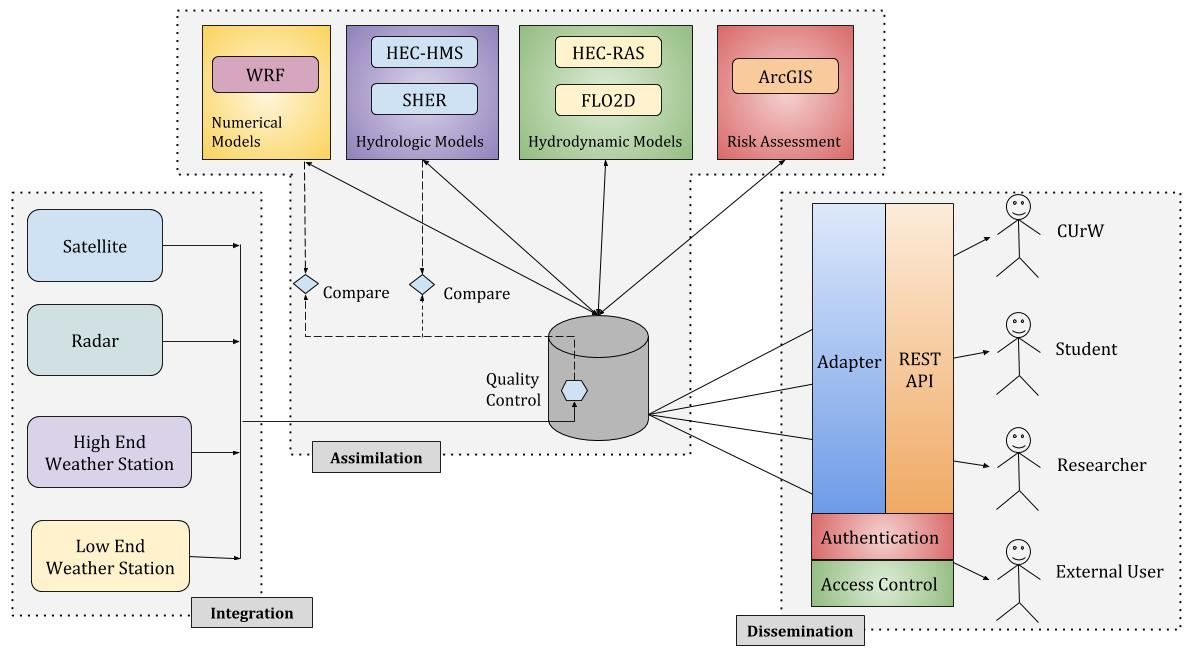
\includegraphics[width=0.5\textwidth]{method/misc/weather_data_system_components.jpg}}
\caption{Components of a weather data system.}
\label{fi:wdia_components}
\end{figure}
\subsubsection{Integration}
The system should capable of integrating data from different source such as satellite data, high end and low end weather station etc. And the system should be able to handle multidimensional spatial and temporal weather data efficiently and optimally. 
\subsubsection{Assimilation}
Then the system should be able to fulfill weather models varying data requirements. Also those models reproduce large set of redundant data, thus system should store the bulk data while optimizing the disk space.
\subsubsection{Dissemination}
Then different users should be able to retrieve data as they required. Also the users should be able to easy to search into the available that in the system base on timeseries metadata or based on Geo queries.

\subsubsection{Timeseries}
A timeseries is simply a series of data points ordered in time. In weather domain, it interest in timeseries in perspective of observations to forecasting.
Each timeseries, the data points can be form in different formats as well.
\begin{itemize} 
    \item Scalar - 0D
    \item Vector - 1D
    \item Grid - 2D
    \item Polygon - 2D
\end{itemize}
    
WDIAS is focus on handling Scalar, Vector and Grid data timeseries via the thesis. But the system is capable of extending to handle polygon timeseries as well.

\subsubsection{Base of WDIAS architecture}
The base of WDIAS architecture origins based on attributes of a timeseries. There are many attributes to differentiate timeseries one from another. But following can be consider as key attributes to uniquely identify a timeseries from another for the \acrshort{wdias}. In detail description available at the section \ref{se:db_struct}.
\begin{itemize}
    \item Module - module that generate the timeseries
    \item Value Type - Scalar, Vector, Grid, Polygon
    \item Location 
    \item Parameter - measuring parameter of timeseries
    \item Timeseries type
    \begin{itemize}
        \item sources - External, Simulated
        \item category - Historical, forecast
    \end{itemize}
    \item Time step
\end{itemize}
